\chapter{*LLM 智能体的机制可解释性}\label{chap:mi}

\begin{learningbox}
本章将介绍如何运用可解释人工智能与机制可解释性的工具，观察大语言模型的黑箱内部。具体而言，学完本章后，你将能够：
\begin{itemize}[leftmargin=*, nosep]
    \item 区分四种主要的可解释性范式：\textit{行为可解释性}、\textit{归因可解释性}、\textit{基于概念的可解释性}与\textit{机制可解释性}。
    \item 解释幻觉与{\em 忠实性}的关系，并说明机制分析方法如何识别导致模型失效的内部回路。
    \item 描述 Transformer 的{\em 残差流}表述，并解释信息如何跨层逐步细化。
    \item 运用{\em Logit 透镜}与调优透镜，将模型预测在各层间的演变过程可视化。
    \item 解释{\em 多义性与叠加}，并理解为什么单个神经元不适合作为解释的基本单位。
    \item 使用{\em 稀疏自编码器}进行字典学习，将模型激活分解为具有单义性、可供人类理解的特征。
    \item 进行{\em 回路分析与激活修补}，识别产生特定模型行为的内部算法，并从因果层面加以验证。
\end{itemize}
\end{learningbox}

\section{打开大语言模型的黑箱}
大语言模型（large language model，LLM）内部是如何运作的？打开大型神经网络架构的黑箱，是一个重要的研究课题。我们希望理解数十亿个神经元如何编码表征、如何推理，以及如何得出结论。可解释人工智能（explainable artificial intelligence，XAI）领域提供了许多不同的方法来研究这些问题 \citep{minh2022explainable,rios2020feature,van2022comparison,selvaraju2017grad,ali2022xai}。

来自经典机器学习领域的静态 XAI 方法已经取得了相当大的成功 \citep{molnar2020interpretable}。已有方法能够解释输入图像如何映射到输出类别，例如使用特征图的方法 \citep{ren2016object,kohonen1982self,redmon2016you}。对于结构化数据，反事实分析 \citep{karimi2020model,explains24}、LIME \citep{ribeiro2016should}、SHAP \citep{lundberg2017unified} 等方法有助于理解输入如何映射到输出。这些方法属于\emph{行为可解释性（behavioral interpretability）}与\emph{归因可解释性（attributional interpretability）}算法，均将模型视为黑箱（图~\ref{fig:MIconcepts}）。SHAP 和 LIME 等归因方法近似估计不同输入特征对最终输出的贡献。反事实方法等所实现的行为分析，则能够帮助我们理解哪些特征起作用，但不一定能说明其作用有多大。

\begin{figure}[!ht]
  \begin{center}
    \begin{tikzpicture}
  \node[anchor=south west, inner sep=0] (miimage) at (0,0)
    {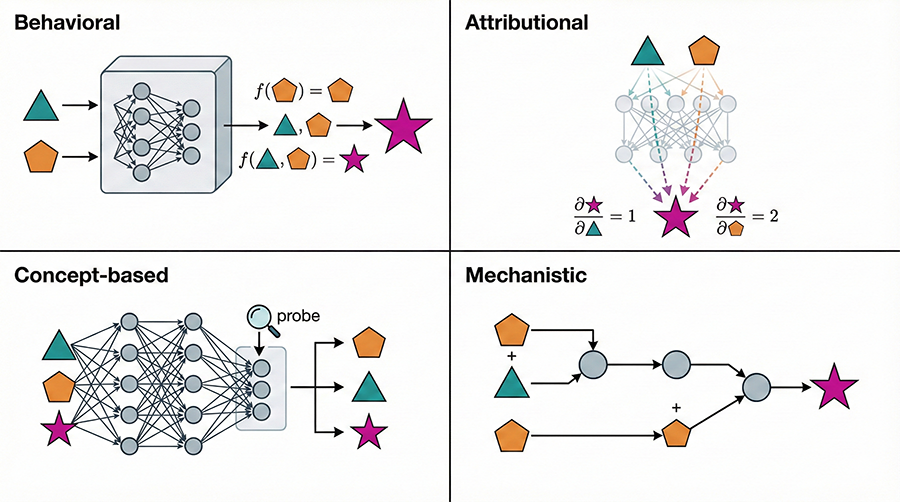
\includegraphics[width=0.96\linewidth]{figures/MI-concepts.png}};
  \begin{scope}[x={(miimage.south east)},y={(miimage.north west)}]
    \fill[white] (0.012,0.923) rectangle (0.488,0.995);
    \fill[white] (0.512,0.923) rectangle (0.990,0.995);
    \fill[white] (0.012,0.418) rectangle (0.488,0.495);
    \fill[white] (0.512,0.418) rectangle (0.990,0.495);
    \node[anchor=north west, font=\small\sffamily\bfseries] at (0.015,0.982) {行为可解释性};
    \node[anchor=north west, font=\small\sffamily\bfseries] at (0.515,0.982) {归因可解释性};
    \node[anchor=north west, font=\small\sffamily\bfseries] at (0.015,0.476) {基于概念的可解释性};
    \node[anchor=north west, font=\small\sffamily\bfseries] at (0.515,0.476) {机制可解释性};
    \fill[white] (0.305,0.348) rectangle (0.367,0.385);
    \node[anchor=west, font=\footnotesize\sffamily] at (0.304,0.367) {探针};
  \end{scope}
\end{tikzpicture}

    \caption{\emph{可解释性范式}的分类。行为可解释性将模型视为黑箱，描绘输入与输出的关系（$f(x) = y$）。归因方法利用梯度或显著性，量化特定输入特征对最终输出的影响。基于概念的可解释性使用探针，在隐藏层中识别可供人类理解的高层表征。机制可解释性则试图对支配模型行为的特定因果回路与内部算法进行逆向工程。\label{fig:MIconcepts}}
  \end{center}
\end{figure}

\emph{基于概念的可解释性（concept-based interpretability）}超越了表层的输入与输出相关性，试图识别模型的内部状态是否编码了特定的、可供人类理解的信息。研究者主要通过\emph{线性探测（linear probing）}开展这类研究：在冻结的隐藏激活上训练一个简单的监督分类器，以检测特定语义概念是否存在，例如词性、情感或事实性实体 \citep{alain2016understanding, belinkov2022probing}。归因方法突出输入的\textit{哪些}部分具有影响力，而探测使研究者能够验证模型在不同层表征了\textit{什么}知识（图~\ref{fig:MIconcepts}）。不过，探测有一个已知局限，即{\em 因果鸿沟（causal gap）}：发现某一层表征了一个概念，并不一定意味着模型在作出最终预测时使用了这一信息。

近来，研究者开发了动态方法，用于揭示大型 Transformer 模型内部的活动模式。这些方法属于机制可解释性（mechanistic interpretability，MI）这一子领域。机制可解释性的目标，是揭示模型动态得出结论的机制 \citep{nanda2023progress,bereska2024mechanistic,ferrando2024primer,rai2024practical}。
换言之，机制可解释性试图从模型的内部激活与连接出发，为其行为提供底层的因果解释，类似于将程序的二进制文件反编译为可读代码。
稀疏自编码器（sparse autoencoder，SAE）\citep{cunningham2023sparse,makelov2024towards}、神经透镜（neural lens）\citep{black2022interpreting}和回路发现（circuit discovery）\citep{conmy2023towards}等方法，已经成功帮助我们更深入地理解大语言模型的运作方式，例如它们如何下国际象棋 \citep{davis2024decoding}。

可解释人工智能，尤其是机制可解释性，是活跃的研究领域，将使我们更好地理解大语言模型如何推理和得出结论 \citep{sharkey2025open}。在获得更深入的理解之后，我们便可以据此改进大语言模型，例如减少幻觉。

本章将深入介绍机制可解释性的多个方面。

\section{模型推理中的幻觉与忠实性}

在高风险环境中部署大语言模型时，一个重大障碍是\emph{幻觉（hallucination）}，即生成句法上看似合理、事实却不正确的内容。从可解释性的角度看，挑战在于区分模型的输出究竟来自可靠的\emph{内部计算}，还是\emph{事后合理化（post-hoc justification）}。这种区别被形式化为对\emph{忠实性（faithfulness）}的研究，即模型所陈述的推理过程，例如思维链提示中的推理，在多大程度上是其最终输出的因果来源。

机制可解释性提供了必要的工具，使我们能够超越准确率等行为指标，从因果角度理解模型的失效模式。例如，利用稀疏自编码器的研究已经识别出特定的\emph{诚实性（honesty）}或\emph{知识检索（knowledge retrieval）}回路 \citep{lindsey2025biology}。在这些研究中，研究者识别出了模型遇到不熟悉的实体时会激活的潜在特征。如果这些回路的抑制逻辑失效，即相关\emph{知识}特征的激活较低，模型却仍然继续生成词元，就会直接导致编造的答案。

此外，机制可解释性使我们能够研究中间推理步骤的\emph{因果必要性（causal necessity）}。模型虽然可能生成令人信服的思维链（chain of thought，CoT），但它仍有可能已经通过另一条内部捷径算出了最终答案，随后只是像\emph{随机鹦鹉（stochastic parrot）}一样生成思维链。

为了检验这一点，\citet{chen2025does} 将\emph{因果中介分析（causal mediation analysis）}与稀疏自编码器结合起来，对算术任务中的潜在思维过程进行干预。他们将启用思维链的一次运行中的潜在激活，注入一次标准的零样本运行，结果表明，在足够大的模型中，这些中间思维显著提高了模型对解答的置信度。这为以下观点提供了实证证据：对于较大的架构，思维链并非仅有表面作用，而是模型推理链中一个\emph{忠实}的因果环节。

相反，较小模型中缺少这类因果联系，表明\emph{忠实推理}可能是一种随规模涌现的性质，只有当模型拥有足够多的参数、能够表征复杂的多步算法时才会出现。开发可靠的指标来量化这种忠实性，是人工智能安全的重要研究前沿。通过观察模型的激活，我们有望开发出幻觉检测器：当模型内部的置信度特征与外部输出的详尽程度不一致时，检测器便会触发。

\section{残差流与迭代细化} \label{residualstream}

在探索具体的机制可解释性方法之前，有必要为 Transformer 架构建立一个形式化的理解框架。在经典前馈网络中，每一层都会替换前一层的表征；现代 Transformer 则在\textit{残差流（residual stream）}上运作 \citep{elhage2021mathematical}。

形式上，令 $h_\ell \in \mathbb{R}^{d_{model}}$ 表示第 $\ell$ 层之后的隐藏表征状态。Transformer 架构由以下递推式定义：
\begin{equation}
    h_\ell = h_{\ell-1} + \mathcal{F}_\ell(h_{\ell-1})
\end{equation}
其中，$\mathcal{F}_\ell$ 表示第 $\ell$ 层执行的计算，包括多头注意力块与前馈块。


这一结构意味着，最终表征 $h_L$ 是初始嵌入 $x_{embed}$ 与随后每一层的贡献（$\Delta h$）的累加和：
\begin{equation}
    h_L = x_{embed} + \sum_{\ell=1}^{L} \Delta h_\ell
\end{equation}

从这一视角看，残差流充当了高维\emph{通信通道}。各层并不变换整个状态，而是从残差流中读取信息，执行局部计算，再通过向量加法将结果写回残差流。这种可加性确保信息能够跨越许多层持续存在；更重要的是，它为模型最终输出的线性分解提供了依据。


\section{多义性与叠加}

\begin{figure}[!ht]
  \begin{center}
    \begin{tikzpicture}
  \node[anchor=south west, inner sep=0] (polyimage) at (0,0)
    {\includegraphics[width=0.84\linewidth]{figures_zh/ch21/polysemanticity_graphics.pdf}};
  \begin{scope}[x={(polyimage.south east)},y={(polyimage.north west)}]
    \node[font=\small\sffamily\bfseries] at (0.526,0.967) {神经元激活空间中的多义性};
    \node[font=\footnotesize\sffamily] at (0.527,0.034) {神经元 A 的激活};
    \node[rotate=90, font=\footnotesize\sffamily] at (0.041,0.503) {神经元 B 的激活};
    \node[anchor=west, font=\footnotesize\sffamily\bfseries] at (0.838,0.275) {概念 1};
    \node[anchor=west, font=\footnotesize\sffamily\bfseries] at (0.259,0.699) {概念 2};
    \node[anchor=west, font=\footnotesize\sffamily\bfseries] at (0.722,0.738) {概念 3};
    \node[anchor=west, font=\footnotesize\sffamily\bfseries] at (0.335,0.468) {概念 4};
    \node[anchor=west, font=\footnotesize\sffamily\bfseries] at (0.645,0.391) {概念 5};
    \node[anchor=north west, inner sep=0, text width=0.420\linewidth,
          font=\footnotesize\sffamily, align=left] at (0.162,0.871) {
      \textbf{多义性：}\\
      单个神经元（坐标轴）参与表征多个不同概念。
      这些概念以激活空间中的“方向”分布，
      而不是与各个坐标轴完全对齐。
    };
  \end{scope}
\end{tikzpicture}

    \caption{大语言模型及其他基于 Transformer 的模型中的多义性概念\label{fig:polysemanticity}}
  \end{center}
\end{figure}

对神经网络进行逆向工程时，一个主要瓶颈是\emph{多义性（polysemanticity）}（图~\ref{fig:polysemanticity}）：经验上，单个神经元经常会对多个语义上互不相关的概念产生激活。这一现象与\emph{叠加（superposition）}密切相关。在叠加状态下，模型表征的特征数为 $n$，而表示空间的维度为 $m$，其中 $n > m$。根据\emph{线性表示假说（linear representation hypothesis）}，模型利用激活空间的高维几何结构，将特征存储为近乎正交的向量。这虽然能够高效压缩信息，却也造成了基底不匹配：固定的神经元基底与真正的特征基底并不对齐。

\citet{elhage2022toy} 对此给出了形式化描述。他们通过简化模型证明，当特征具有稀疏性时，叠加是模型最大化信息密度的一种有数学依据的策略。他们还在特征编码中发现了\emph{相变（phase transition）}：随着概念的稀疏性增加，模型可以将更多特征压入相同数量的维度，不过代价是这些特征之间会出现干扰或噪声。

为了解开这种纠缠，研究者转向\emph{字典学习（dictionary learning）}，其中最具代表性的方法是\emph{稀疏自编码器}。其目标是学习一个线性变换，将相互纠缠的神经元激活映射到维度高得多的稀疏潜在空间。\citet{bricken2023monosemanticity} 成功将这一方法应用于小规模 Transformer，证明所得到的 SAE 特征比原始神经元具有显著更强的单义性（monosemanticity），也更容易被人类理解。这表明，模型并非天生不可解释，而是我们一直在通过错误的坐标系观察它们。

后续工作探索了能否通过修改架构，缓解多义性的出现。例如，\citet{liu2023seeing} 等研究者考察了不同的激活函数或正则化惩罚项，例如 $L_1$ 稀疏性，如何促使模型采用更对齐、更可解释的内部基底。尽管取得了这些进展，多义性仍然是最先进模型中普遍存在的挑战。机制可解释性领域目前的共识是：解释模型需要超越“以神经元为单位”的范式，转而识别模型实际执行因果逻辑计算所依赖的底层\emph{稀疏特征基底}。




\section{Logit 透镜}

机制可解释性的一个基本直觉是，Transformer 模型并不是在最后一层一步完成输出计算的。相反，它在\emph{残差流}中逐步细化表征。\textit{Logit 透镜（logit lens）}\footnote{这一方法最初发表于以下博客文章：\url{https://www.lesswrong.com/posts/AcKRB8wDpdaN6v6ru/interpreting-gpt-the-logit-lens}。\citep{wang2025logitlens4llmsextendinglogitlens} 提供了更新后的实现。}将中间层的隐藏状态直接解码到输出词表空间，为我们观察这一过程提供了一扇窗口。

\subsection{形式化机制}
考虑一个具有 $L$ 层的 Transformer。令 $x_0$ 表示某个词元的初始嵌入，$h_\ell$ 表示第 $\ell \in \{1, \dots, L\}$ 层之后的残差流状态。在标准前向传播中，最终隐藏状态 $h_L$ 被转换为 logit $y$；这一过程使用层归一化（layer norm，LN）与反嵌入矩阵（unembedding matrix）$W_U \in \mathbb{R}^{d_{model} \times |V|}$：
\begin{equation}
    y = \text{Softmax}(\text{LN}(h_L) W_U)
\end{equation}
Logit 透镜将这一过程推广到中间状态 $h_\ell$，对其应用\emph{相同的}反嵌入变换：
\begin{equation}
    \hat{y}_\ell = \text{Softmax}(\text{LN}(h_\ell) W_U)
\end{equation}
其中，$\hat{y}_\ell$ 表示模型在第 $\ell$ 层的暂定概率分布。将所有层的这些分布可视化，研究者便可以观察\emph{信念的演变}，即模型如何从模糊的语义簇逐渐转向对具体词元的预测。

\begin{figure}[!ht]
    \centering
    \begin{tikzpicture}[
    node distance=1.2cm and 2cm,
    layer/.style={rectangle, draw, fill=gray!10, minimum width=3cm, minimum height=0.8cm, font=\small\sffamily, rounded corners=2pt},
    stream/.style={-{Stealth}, line width=1.5pt, color=black!45},
    lens_path/.style={-{Stealth}, line width=1.2pt, color=teal, dashed},
    box/.style={rectangle, draw, fill=white, font=\footnotesize\sffamily, inner sep=4pt, rounded corners=1pt},
    lens_box/.style={rectangle, draw=teal!70!purple, fill=teal!5, thick, font=\footnotesize\sffamily, inner sep=5pt, rounded corners=1pt, align=center},
    prob_plot/.style={thin, fill=teal!60},
    lens_style/.style={circle, draw=teal!80, fill=teal!5, thick, minimum size=0.6cm},
    handle_style/.style={draw=teal!80, line width=2pt, cap=round}
]

    \node (input) at (0,0) [font=\small\sffamily] {输入：``The''};

    \node (layer1) [layer, above=of input] {第 1 层};
    \node (layer2) [layer, above=0.8cm of layer1] {第 2 层};
    \node (dots)   [above=0.4cm of layer2, font=\boldmath] {$\vdots$};
    \node (layerL) [layer, above=0.4cm of dots] {第 $L$ 层};
    \node at ($(layer1.east)+(0.2,-0.2)$) [rotate=90, font=\footnotesize\sffamily\bfseries, color=black!45, anchor=west] {残差流};

    \draw [stream] (input) -- (layer1);
    \draw [stream] (layer1) -- (layer2);
    \draw [stream] (layer2) -- (dots);
    \draw [stream] (dots) -- (layerL);

    \node (final_ops) [box, above=0.8cm of layerL, align=center] {层归一化 \\ + $W_U$ + Softmax};
    \draw [stream] (layerL) -- (final_ops);


    \node (final_plot) [above=0.5cm of final_ops, minimum width=2cm, minimum height=1cm] {};
    \begin{scope}[shift={(final_plot.south west)}, xscale=0.5, yscale=0.8]
        \draw[->, thin] (0,0) -- (4.5,0);
        \draw[->, thin] (0,0) -- (0,1.2);
        \foreach \x/\y/\c in {0.5/0.1/gray, 1.5/0.9/magenta, 2.5/0.05/gray, 3.5/0.2/gray} { \draw[fill=\c!50] (\x-0.2,0) rectangle (\x+0.2,\y); }
         \node at (1.5, 1.1) [font=\footnotesize\sffamily, color=magenta!80] {``cat''};
    \end{scope}
    \node [right=0.1cm of final_plot, font=\footnotesize\sffamily, align=left] {模型最终\\预测 $y$};


    \coordinate (tap_point) at ($(layer2.north)!0.5!(dots.south)$);

    \begin{scope}[shift={($(tap_point)+(1.8,0.9)$)}]
        \draw[handle_style] (-0.2,-0.2) -- (0,0);
        \node (glass) [lens_style] at (0.2,0.2) {};
        \draw[white, line width=1pt, cap=round] (0.3,0.3) arc (45:100:0.15);

        \node (lens_text) [right=0.1cm of glass, font=\small\sffamily\bfseries, color=teal!80] {Logit 透镜};
    \end{scope}


    \node (lens_transform) [lens_box, right=2.6cm of tap_point] {层归一化 \\ + $W_U$ + Softmax};

    \draw[lens_path] (tap_point) -- (lens_transform.west);


    \node (lens_plot) [right=0.5cm of lens_transform, minimum width=2cm, minimum height=1cm] {};
    \begin{scope}[shift={(lens_plot.south west)}, xscale=0.5, yscale=0.8]
        \draw[->, thin] (0,0) -- (4.5,0);
        \draw[->, thin] (0,0) -- (0,1.2);
        \foreach \x/\y/\c in {0.5/0.4/gray, 1.5/0.7/gray, 2.5/0.8/blue!70!purple, 3.5/0.1/gray} {
             \draw[fill=\c!50] (\x-0.2,0) rectangle (\x+0.2,\y);
        }
         \node at (2.5, 1.0) [font=\footnotesize\sffamily, color=blue!70!purple] {``dog''};
    \end{scope}
    \node [below=0.1cm of lens_plot, font=\footnotesize\sffamily, align=center, color=blue!70!purple] {透镜输出 $\hat{y}_\ell$};

\end{tikzpicture}

    \caption{\emph{Logit 透镜}的可视化。在某个中间层，例如第 2 层，截取残差流，并使用模型最终的反嵌入矩阵（$W_U$）进行解码。这揭示了模型在该步骤的当前信念，不过早期层的结果可能带有较多噪声。}
    \label{fig:logit_lens}
\end{figure}


\paragraph{直接 logit 归因}
Logit 透镜提供了残差流 $h_\ell$ 的整体视图，但我们常常希望单独考察\emph{某一}层或某一注意力头的贡献。由于最终 logit $y$ 是各层输出累加和的线性函数，我们可以将第 $\ell$ 层的特定输出 $\Delta h_\ell$ 直接投影到词表空间，计算该层的\emph{直接 logit 归因（direct logit attribution，DLA）}：
\begin{equation}
    \text{DLA}(\ell) = \text{LN}(\Delta h_\ell) W_U
\end{equation}
直接 logit 归因使研究者能够确定，究竟是哪些组件在向残差流写入正确答案，而不只是识别答案在哪里开始可见。在事实回忆研究中，直接 logit 归因经常揭示：正确词元的概率增幅，绝大部分来自某一个产生知识的层。

\subsection{从 Logit 透镜到调优透镜}
最初的 Logit 透镜对于网络最后三分之一的层能够提供丰富信息，但在早期层往往会产生无意义的输出，或高熵分布。这是因为，例如第 2 层的残差流尚未形成适合输出分布的表示形式；它可能还在存储低层的位置相关信息，而这些信息在数学上与反嵌入矩阵 $W_U$ 正交。

\begin{figure}[htbp]
    \centering
    \begin{tikzpicture}[
    node distance=1.2cm and 2cm,
    layer/.style={rectangle, draw, fill=gray!10, minimum width=3cm, minimum height=0.8cm, font=\small\sffamily, rounded corners=2pt},
    stream/.style={-{Stealth}, line width=1.5pt, color=black!45},
    lens_path/.style={-{Stealth}, line width=1.2pt, color=teal, dashed},
    tuned_path/.style={-{Stealth[scale=1.2]}, line width=1.5pt, color=blue!70!purple, dashed},
    tuned_box/.style={rectangle, draw=blue!70!purple, fill=blue!5, thick, font=\footnotesize\sffamily, inner sep=5pt, rounded corners=1pt, align=center},
    box/.style={rectangle, draw, fill=white, font=\footnotesize\sffamily, inner sep=4pt, rounded corners=1pt},
    prob_plot/.style={thin, fill=teal!60},
    lens_style/.style={circle, draw=blue!80!purple, fill=purple!5, thick, minimum size=0.6cm},
    handle_style/.style={draw=blue!80!purple, line width=2pt, cap=round}
]

    \node (input) at (0,0) [font=\small\sffamily] {输入：``The''};

    \node (layer1) [layer, above=of input] {第 1 层};
    \node (layer2) [layer, above=0.8cm of layer1] {第 2 层};
    \node (dots)   [above=0.4cm of layer2, font=\boldmath] {$\vdots$};
    \node (layerL) [layer, above=0.4cm of dots] {第 $L$ 层};
    \node at ($(layer1.east)+(0.2,-0.2)$) [rotate=90, font=\footnotesize\sffamily\bfseries, color=black!45, anchor=west] {残差流};

    \draw [stream] (input) -- (layer1);
    \draw [stream] (layer1) -- (layer2);
    \draw [stream] (layer2) -- (dots);
    \draw [stream] (dots) -- (layerL);

    \node (final_ops) [box, above=0.8cm of layerL, align=center] {层归一化 \\ + $W_U$ + Softmax};
    \draw [stream] (layerL) -- (final_ops);


    \node (final_plot) [above=0.5cm of final_ops, minimum width=2cm, minimum height=1cm] {};
    \begin{scope}[shift={(final_plot.south west)}, xscale=0.5, yscale=0.8]
        \draw[->, thin] (0,0) -- (4.5,0);
        \draw[->, thin] (0,0) -- (0,1.2);
        \foreach \x/\y/\c in {0.5/0.1/gray, 1.5/0.9/magenta, 2.5/0.05/gray, 3.5/0.2/gray} { \draw[fill=\c!50] (\x-0.2,0) rectangle (\x+0.2,\y); }
         \node at (1.5, 1.1) [font=\footnotesize\sffamily, color=magenta!80] {``cat''};
    \end{scope}
    \node [above right=0.12cm and 0.1cm of final_plot, font=\footnotesize\sffamily, align=left] {模型最终\\预测 $y$};



    \coordinate (tap_point) at ($(layer2.north)!0.5!(dots.south)$);

    \begin{scope}[shift={($(tap_point)+(1.8,0.8)$)}]
        \draw[handle_style] (-0.2,-0.2) -- (0,0);
        \node (glass) [lens_style] at (0.2,0.2) {};
        \draw[white, line width=1pt, cap=round] (0.3,0.3) arc (45:100:0.15);

        \node (lens_text) [right=0.1cm of glass, font=\small\sffamily\bfseries, color=blue!80!purple] {调优透镜};
    \end{scope}

    \coordinate (tap_point) at ($(layer2.north)!0.5!(dots.south)$);

    \node (tuned_transform) [tuned_box, right=2.2cm of tap_point] {学习得到的\\仿射变换 \textbf{$\phi_2(h_2)$}};

    \draw[tuned_path] (tap_point) -- (tuned_transform.west);

    \node (tuned_softmax) [tuned_box, right=0.8cm of tuned_transform] {Softmax};
    \draw[tuned_path] (tuned_transform) -- (tuned_softmax);

    \node (lens_plot) [right=0.5cm of tuned_softmax, minimum width=2cm, minimum height=1cm] {};
    \begin{scope}[shift={(lens_plot.south west)}, xscale=0.5, yscale=0.8]
        \draw[->, thin] (0,0) -- (4.5,0);
        \draw[->, thin] (0,0) -- (0,1.2);
        \foreach \x/\y/\c in {0.5/0.15/gray, 1.5/0.7/blue!70!purple, 2.5/0.1/gray, 3.5/0.1/gray} {
             \draw[fill=\c!50] (\x-0.2,0) rectangle (\x+0.2,\y);
        }
         \node at (1.5, 0.9) [font=\footnotesize\sffamily, color=blue!70!purple] {``cat''};
    \end{scope}
    \node [below=0.1cm of lens_plot, font=\footnotesize\sffamily, align=center, color=blue!70!purple] {调优输出 $y_{tuned,2}$};

    \draw[->, dashed, thick, color=black!60, bend left=45] (final_plot.east) to node[midway, right, xshift=0.45cm, font=\footnotesize\sffamily, align=center] {训练信号\\（最小化 KL 散度）} (tuned_transform.south east);

\end{tikzpicture}

    \caption{\textit{调优透镜}的可视化。这一方法使用针对各层\emph{学习得到的}变换（$\phi_\ell$）来解码残差流。相较于朴素透镜，该变换通过训练将中间表征与最终输出分布对齐，从而更清楚地呈现早期层中信息涌现的过程。}
    \label{fig:tuned_lens}
\end{figure}

为了弥合这一差距，\citet{belrose2023eliciting} 提出了\textit{调优透镜（tuned lens）}。调优透镜不使用静态的 $W_U$，而是为各层训练一个仿射变换 $\phi_\ell$，将 $h_\ell$ 映射到 logit 空间：
\begin{equation}
    y_{tuned, \ell} = \text{Softmax}(\phi_\ell(h_\ell))
\end{equation}
通过训练，变换 $\phi_\ell$ 使 $y_{tuned, \ell}$ 与模型实际的最终输出 $y$ 之间的 KL 散度最小化。这实际上将早期层的内部语言翻译成了输出词表，揭示出事实信息在网络中的出现时间，往往比朴素 Logit 透镜所显示的早得多。

\subsection{应用与解读}
透镜是重要的诊断工具，可用于识别适合\emph{提前退出（early exit）}的层，并定位特定的知识神经元。例如，如果某个事实，如 Paris，对应的 logit 在第 14 层从第 100 名跃升到第 1 名，这就表明，第 14 层的注意力头或多层感知机子层可能负责检索这一事实。

\emph{注意力透镜（attention lens）}\citep{sakarvadia2023attention}等变体将类似的逻辑应用于单个注意力头的输出，使我们能够单独观察每个头对预测的贡献。这些工具共同推动我们改变对 Transformer 的看法：从顺序执行的流程，转向对潜在信息进行\emph{累加式迭代细化}的系统。



\section{回路分析}

机制可解释性的一个核心目标是识别\emph{回路（circuit）}：它是模型计算图中实现某个特定高层功能所必需且充分的最小子图。回路发现与行为分析不同，它试图解释信息从输入嵌入到最终 logit 的逐步变换\emph{如何}发生。

\subsection{典型回路：归纳头}
\emph{归纳头（induction head）}的发现是 Transformer 可解释性研究的一个里程碑 \citep{olsson2022context}。归纳头是一种由至少两个注意力头组成的专门回路，用于实现前缀匹配算法。形式上，给定序列 $[A][B] \dots [A]$，当前位置 $[A]$ 的归纳头会关注此前出现的 $[A]$，并将其后的词元 $[B]$ \emph{复制}到残差流中（图~\ref{fig:induction_head}）。

\paragraph{组合机制}
为了理解归纳回路中的两个头如何通信，我们必须定义三种\emph{注意力组合（attention composition）}\citep{elhage2021mathematical}：
\begin{itemize}
    \item V 组合（V-Composition）：前一个头的输出，即值（Value），用作后一个头的输入。
    \item Q 组合／K 组合（Q-Composition／K-Composition）：前一个头通过向词元的查询（Query）向量或键（Key）向量写入信息，影响后一个头关注\emph{哪里}。
\end{itemize}
归纳头通常依赖\emph{K 组合}：早期层中的前一词元头（previous token head）将有关前一词元的信息写入残差流。随后，较后层中的归纳头在自己的键向量中使用这些信息来匹配当前前缀，从而关注历史中正确的词元 $[B]$。

\begin{figure}[htbp]
    \centering
    \begin{tikzpicture}[
    node distance=0pt,
    token/.style={
        rectangle,
        draw=gray!50,
        thick,
        minimum height=0.9cm,
        text depth=0.3ex,
        text height=0.8em,
        font=\sffamily\small,
        inner xsep=4pt,
        outer sep=0pt,
        anchor=west
    },
    red_highlight/.style={fill=red!40},
    purple_highlight/.style={fill=blue!30!purple!40},
    grey_border/.style={draw=gray!90, line width=1.5pt},
    attention_arrow/.style={
        ->,
        >={Stealth[length=3mm, width=2mm]},
        color=red!60,
        line width=1.5pt,
        font=\sffamily\small,
        cap=round
    },
    label_text/.style={
        font=\sffamily\small,
        color=darkgray!70,
        align=left
    },
    bold_label/.style={
        font=\sffamily\bfseries,
        color=gray!90
    }
]

\node[font=\sffamily\small, color=black!65, anchor=south west] at (0, 0.85) {随机词元};
\node[token] (t1_1) at (0,0) {Category};
\node[token] (t1_2) at (t1_1.east) {40};
\node[token] (t1_3) at (t1_2.east) {ids};
\node[token] (t1_4) at (t1_3.east) {node};
\node[token, red_highlight] (t1_5) at (t1_4.east) {struction};

\node[font=\sffamily\small, color=black!65, right=0.5cm of t1_5] (ellipsis) {...};

\node[font=\sffamily\small, color=black!65, anchor=south west] at ($(ellipsis.east)+(0.5, 0.85)$) {随机词元的重复};
\node[token, right=0.5cm of ellipsis] (t2_1) {Category};
\node[token] (t2_2) at (t2_1.east) {40};
\node[token] (t2_3) at (t2_2.east) {ids};
\node[token, grey_border] (t2_4) at (t2_3.east) {node};
\node[token, purple_highlight] (t2_5) at (t2_4.east) {struction};

\draw[attention_arrow] (t2_4.north) to[out=90, in=90, looseness=0.8] node[above=0.15cm] {注意力} (t1_5.north);



\draw[gray!50, thick] (t1_4.south) -- ++(0,-0.8cm) coordinate (l1_line);
\node[label_text, below=0.1cm of l1_line, anchor=north, text width=4.0cm, align=center] {
    被关注词元的{\bfseries 前缀}\\
    = 当前词元
};

\draw[gray!50, thick] (t2_5.south) -- ++(0,-0.8cm) coordinate (l2_line);
\node[label_text, below=0.1cm of l2_line, anchor=north east, xshift=0.8cm, text width=5.5cm] {
    {\bfseries 复制}被关注的词元。下一词元的\\
    对应 \colorbox{blue!30!purple!40}{\strut logit} 随之增大。
};

\end{tikzpicture}

    \caption{\emph{归纳头回路的运作机制。}归纳头实现了一种前缀匹配算法：模型识别出当前词元，即前缀，在此前出现的位置，并关注其后的词元，以预测重复序列。
    \label{fig:induction_head} }
\end{figure}

\citet{olsson2022context} 观察到，这些头会在训练中的某个特定相变阶段涌现，同时模型的上下文学习能力也会急剧提升。这是最早将复杂能力追溯到跨越多个层实现的某个具体、离散算法的实例之一。

\subsection{回路发现的方法}
手动识别回路需要大量人力。\citet{wang2022interpretability} 对\emph{间接宾语识别（indirect object identification，IOI）}任务的研究，至今仍是手动追踪的典范。他们利用\emph{路径修补（path patching）}，识别出了一个包含 26 个注意力头的网络，这些头按照作用被分为{\em 姓名搬运头（Name Movers）}、{\em S 抑制头（S-Inhibition Heads）}和{\em 重复词元检测器（Duplicate Token Detectors）}等，共同完成共指消解。\emph{共指消解（coreference resolution）}是识别文本中不同词元何时指向同一个实体的过程。例如，在 IOI 任务中，模型必须确定，后面提到的某个姓名，即间接宾语，指回句子前面引入的某个人；这一计算由注意力头组成的专门子网络实现。

不过，要将这些发现推广到前沿模型，就需要\emph{自动回路发现（automated circuit discovery，ACD）}。
\begin{itemize}
    \item 自动回路发现：\citet{conmy2023towards} 提出了一种算法，通过递归消融对计算图中的边进行剪枝，只保留那些一旦移除，就会显著降低模型在特定任务上表现的边。
    \item 稀疏特征回路（Sparse Feature Circuits）：近年来的框架超越了神经元，整合稀疏自编码器，在\emph{特征空间}中而非神经元空间中追踪回路 \citep{marks2024sparse}。研究者将 SAE 特征视为节点，将特征之间的权重视为边，由此构建归因图，将可供人类理解的概念流动过程可视化，例如\emph{拒绝}、\emph{翻译}或\emph{语法检查}。
\end{itemize}



\paragraph{评估：忠实性、完整性与最小性}
区分\emph{推测的}回路与\emph{因果}回路至关重要。如果将回路之外的所有组件消融后，模型的表现仍然保持不变，就认为该回路具有\emph{忠实性}。如果回路涵盖了模型解决任务时使用的全部路径，就认为它具有\emph{完整性（completeness）}。

随着模型规模增大，我们发现算法往往以冗余的方式表示，或分布在残差流的不同位置。因此，回路追踪并非只是寻找一根连线，而是试图描绘信息如何通过模型的高维潜在空间实现\emph{因果中介}。


\section{激活修补与因果干预}

Logit 透镜或探测等观测工具能够识别内部状态与输出之间的相关性，而\emph{激活修补（activation patching）}，也称\emph{因果追踪（causal tracing）}或\emph{互换干预（interchange intervention）}，使研究者能够作出明确的因果论断。这项技术是\emph{因果中介分析}的一种实际应用 \citep{vig2020investigating}，旨在分离出特定模型组件对下游行为的影响（图~\ref{fig:activation_patching}）。

\begin{figure}[htbp]
    \centering
    \begin{tikzpicture}[
    node distance=1.2cm and 2.5cm,
    layer/.style={rectangle, draw, fill=gray!10, minimum width=2.5cm, minimum height=0.7cm, font=\small\sffamily, rounded corners=2pt},
    stream/.style={-{Stealth}, line width=1.5pt},
    clean_color/.style={color=green!60!black},
    corr_color/.style={color=red!60!black},
    patch_color/.style={color=blue!70, dashed, line width=2pt},
    box/.style={rectangle, draw, font=\footnotesize\sffamily, inner sep=4pt, rounded corners=1pt, fill=white}
]

    \node (in_clean) at (0,0) [font=\small\sffamily\bfseries, clean_color] {干净输入 ($x_{clean}$)};
    \node (l1_clean) [layer, above=of in_clean] {第 1 层};
    \node (l2_clean) [layer, above=of l1_clean, draw=green!60!black, fill=green!5, thick] {组件 $z_{i, \ell}$};
    \node (l3_clean) [layer, above=of l2_clean] {第 3 层};
    \node (out_clean) [above=of l3_clean, clean_color, font=\small\sffamily\bfseries] {正确输出};

    \draw [stream, clean_color] (in_clean) -- (l1_clean);
    \draw [stream, clean_color] (l1_clean) -- (l2_clean);
    \draw [stream, clean_color] (l2_clean) -- (l3_clean);
    \draw [stream, clean_color] (l3_clean) -- (out_clean);

    \node (in_corr) at (5,0) [font=\small\sffamily\bfseries, corr_color] {扰乱输入 ($x_{corr}$)};
    \node (l1_corr) [layer, above=of in_corr] {第 1 层};
    \node (l2_corr) [layer, above=of l1_corr, dashed, draw=red!60!black] {已消融／含噪声};
    \node (l3_corr) [layer, above=of l2_corr] {第 3 层};
    \node (out_corr) [above=of l3_corr, blue!70!black, font=\small\sffamily\bfseries] {输出恢复？};

    \draw [stream, corr_color] (in_corr) -- (l1_corr);
    \draw [stream, corr_color] (l1_corr) -- (l2_corr);
    \draw [stream, corr_color] (l2_corr) -- (l3_corr);
    \draw [stream, corr_color] (l3_corr) -- (out_corr);

    \draw [patch_color, -{Stealth[scale=1.5]}] (l2_clean.east) to[bend left=20]
        node[midway, above, font=\footnotesize\sffamily\bfseries, color=blue!70] {修补激活}
        (l2_corr.west);

    \node [below left=0.1cm and 0.1cm of l2_clean, font=\footnotesize\sffamily, color=green!60!black] {信息来源};
    \node [below right=0.1cm and 0.1cm of l2_corr, font=\footnotesize\sffamily, color=red!60!black] {干预目标};

    \node at (2.5, 6) [box, align=center, draw=blue!70] {测量目标概率\\的变化};

\end{tikzpicture}

    \caption{\emph{激活修补。}将模型成功完成任务的\emph{干净运行}中的激活，替换到模型未能完成任务的\emph{扰乱运行}中。通过观察这一互换干预是否恢复正确输出，我们可以从因果层面验证，修补的组件是否负责该特定推理任务。}
    \label{fig:activation_patching}
\end{figure}


\paragraph{形式化框架}
该过程涉及两次不同的前向传播：
\begin{enumerate}
    \item 干净运行（clean run，$x_{clean}$）：使用能够产生目标行为的输入，例如{\em 埃菲尔铁塔位于\textbf{巴黎}}。
    \item 扰乱／反事实运行（corrupted/counterfactual run，$x_{corr}$）：使用经修改、使目标行为消失的输入，例如{\em 罗马斗兽场位于\textbf{罗马}}，或向{\em 埃菲尔铁塔}的嵌入添加高斯噪声。
\end{enumerate}

令 $z_{i, \ell}$ 表示组件 $i$ 在第 $\ell$ 层的激活。在激活修补中，我们在扰乱的前向传播期间，将激活 $z^{corr}_{i, \ell}$ 替换为 $z^{clean}_{i, \ell}$，由此计算一次\emph{修补运行（patched run）}。随后测量\emph{概率恢复程度（probability recovery）}：
\begin{equation}
    \text{Effect} = \frac{P(y_{target} | \text{patched}) - P(y_{target} | \text{corr})}{P(y_{target} | \text{clean}) - P(y_{target} | \text{corr})}
\end{equation}
Effect 得分接近 1.0，表示修补的组件是所研究信息的一个充分的因果中介。


\paragraph{定位知识与回路}
激活修补带来了关于模型架构的重要认识。\citet{meng2022locating} 利用大规模修补扫描，证明事实关联往往集中在模型中间层的特定多层感知机块中。他们发现，即使输入上下文受到扰乱，修补这些\emph{知识神经元（knowledge neuron）}也能够迫使模型输出特定事实。

除了定位之外，修补还是\emph{路径修补}的主要工具，可用于识别组件之间的交互。在前面提到的间接宾语识别研究中，\citet{wang2022interpretability} 修补特定的注意力头，追踪信息如何从{\em 重复词元检测器}流向{\em 姓名搬运头}。这揭示了模型的\emph{计算图}，超越了简单定位，进一步帮助我们理解内部算法。

\paragraph{可扩展性与归因修补}
激活修补的一个主要挑战是计算成本，因为完整扫描需要为模型中的每个组件都进行一次前向传播。为缓解这一问题，研究者使用\emph{归因修补（attribution patching）}\citep{syed2024attribution}，利用梯度对修补效果进行线性近似。这使研究者能够快速提出假设，随后再用精确但较慢的激活修补，验证最有希望的因果候选组件。这种如外科手术般的精确性，使修补成为机制可解释性工具中不可或缺的一部分，帮助研究从推测性解释走向严格的因果证明。


\section{稀疏自编码器：用于特征发现的字典学习}

正如讨论叠加时所述，神经网络表征的特征数往往超过其维度数（$n > d$）。为了解开这种相互纠缠的表征，我们使用\emph{稀疏自编码器}。它是一种无监督字典学习方法，旨在将激活投影到维度更高的稀疏潜在空间，使其中的特征近似具有单义性。

\begin{figure}[htbp]
    \centering
    \begin{tikzpicture}[
    node distance=2cm,
    neuron/.style={circle, draw=gray!70, fill=white, minimum size=0.65cm, thick},
    active_feature/.style={circle, draw=teal!80, fill=teal!20, minimum size=0.65cm, thick, font=\bfseries\tiny},
    inactive_feature/.style={circle, draw=gray!30, fill=gray!5, minimum size=0.6cm, thin},
    flow_arrow/.style={-{Stealth[scale=1.2]}, line width=1.2pt, color=gray!70},
    loss_arrow/.style={-{Stealth[scale=1.2]}, line width=1.5pt, dashed},
    layer_label/.style={font=\sffamily\small\bfseries, align=center},
    math_label/.style={font=\footnotesize\sffamily}
]

    \coordinate (input_col) at (0,0);
    \foreach \i in {1,2,3} {
        \node[neuron] (x\i) at ($(input_col)+(0, -\i*1.2)$) {$x_{\i}$};
    }
    \node[below=0.3cm of x3, font=\bfseries] (x_dots) {$\vdots$};
    \node[neuron, below=0.3cm of x_dots] (xd) {$x_d$};

    \node[layer_label, above=0.5cm of x1] (input_lbl) {输入激活\\$x \in \mathbb{R}^d$};
    \draw[decorate, decoration={brace, amplitude=5pt, mirror}, thick, gray]
        ($(x1.west)+(-0.5,0)$) -- ($(xd.west)+(-0.5,0)$) node[midway, left=0.3cm, font=\sffamily\small] {低维 $d$};


    \coordinate (hidden_col) at (5, 1);
    \foreach \i in {1,2,4,5,7,8} {
        \node[inactive_feature] (c\i) at ($(hidden_col)+(0, -\i*0.8)$) {};
    }
    \node[active_feature] (c3) at ($(hidden_col)+(0, -3*0.8)$) {$c_3$};
    \node[active_feature] (c6) at ($(hidden_col)+(0, -6*0.8)$) {$c_6$};

    \node[below=0.2cm of c8, font=\bfseries] (c_dots) {$\vdots$};
    \node[inactive_feature, below=0.2cm of c_dots] (cN) {};

    \node[layer_label, above=0.5cm of c1] (hidden_lbl) {稀疏潜在特征\\$c \in \mathbb{R}^N$};
    \draw[decorate, decoration={brace, amplitude=5pt}, thick, gray]
        ($(c1.east)+(0.5,0)$) -- ($(cN.east)+(0.5,0)$) node[pos=0.10, right=0.3cm, font=\sffamily\small, align=center] {高维 $N$\\($N \gg d$)};
    \node[right=1.2cm of c_dots, font=\sffamily\footnotesize, color=teal, align=center] {大部分为零\\（稀疏）};


    \coordinate (output_col) at (10,0);
    \foreach \i in {1,2,3} {
        \node[neuron] (hx\i) at ($(output_col)+(0, -\i*1.2)$) {$\hat{x}_{\i}$};
    }
    \node[below=0.3cm of hx3, font=\bfseries] (hx_dots) {$\vdots$};
    \node[neuron, below=0.3cm of hx_dots] (hxd) {$\hat{x}_d$};

    \node[layer_label, above=0.5cm of hx1] (output_lbl) {重构\\$\hat{x} \in \mathbb{R}^d$};



    \node at ($(input_lbl.east)!0.5!(hidden_lbl.west)+(0,0.2)$) [font=\sffamily\small, align=center, inner sep=2pt] {编码器 $W_{enc}$\\+ 稀疏性（如 ReLU）};
    \foreach \inputnode in {x1,x2,x3,xd} {
        \draw[flow_arrow, opacity=0.45] (\inputnode) -- (c3);
        \draw[flow_arrow, opacity=0.45] (\inputnode) -- (c6);
    }

    \node at ($(hidden_lbl.east)!0.5!(output_lbl.west)+(0,0.2)$) [font=\sffamily\small, align=center] {解码器 $W_{dec}$};
    \foreach \outputnode in {hx1,hx2,hx3,hxd} {
        \draw[flow_arrow, opacity=0.6] (c3) -- (\outputnode);
        \draw[flow_arrow, opacity=0.6] (c6) -- (\outputnode);
    }


    \coordinate (bottom_level) at (0, -7.5);

    \draw[loss_arrow, color=red!70, <->] ($(xd.south)+(0,-0.5)$) to[bend right=15]
        node[pos=0.23, below=0.3cm, align=center, font=\sffamily\small, color=red!80] {\textbf{重构损失：}\\$\|x - \hat{x}\|^2$}
        ($(hxd.south)+(0,-0.5)$);

    \draw[loss_arrow, ->, color=blue!70] ($(cN.south)+(0,-2.0)$) --
        node[midway, right, font=\sffamily\small, color=blue!80, align=left] {\textbf{稀疏性惩罚：}\\$+ \lambda \|c\|_1$}
        ($(cN.south)+(0,-0.1)$);

\end{tikzpicture}

    \caption{\emph{稀疏自编码器架构。}模型将较低维的输入激活（$x \in \mathbb{R}^d$）投影到维度高得多的潜在空间（$c \in \mathbb{R}^N$，其中 $N \gg d$）。稀疏性惩罚，例如 $L_1$ 正则化对 $c$ 的约束，迫使大部分隐藏单元保持不活跃状态（灰色），形成一组稀疏的、活跃且可解释的特征（蓝绿色），用于重构原始输入。\label{fig:sae_architecture}}

\end{figure}

\paragraph{形式化架构与训练目标}
稀疏自编码器由编码器与解码器组成。编码器将模型激活 $x \in \mathbb{R}^d$ 映射到高维隐藏状态 $c \in \mathbb{R}^N$，其中 $N \gg d$；解码器则尝试重构原始激活（图~\ref{fig:sae_architecture}）。

编码器通常定义为：
\begin{equation}
    c = \text{ReLU}(W_{enc}(x - b_{dec}) + b_{enc})
\end{equation}
重构结果为：
\begin{equation}
    \hat{x} = W_{dec} c + b_{dec}
\end{equation}

为了确保模型学到的是\emph{稀疏}字典，而非简单的恒等映射，我们优化一个将重构保真度与诱导稀疏性的惩罚项结合起来的损失函数：
\begin{equation}
    \mathcal{L} = \|x - \hat{x}\|^2 + \lambda \|c\|_1
\end{equation}
其中，$\lambda$ 控制重构准确性与特征稀疏性之间的权衡。近期的进展，例如 \emph{JumpReLU 稀疏自编码器}\citep{rajamanoharan2024jumping}，使用带阈值的激活函数，使特征呈现近乎二元的开关行为，更接近离散语义特征的理论理想形式。


\subsection{单义性与影子模型}
稀疏自编码器的有效性已经在不同规模上得到验证。\citet{cunningham2023sparse} 证明，稀疏自编码器能够恢复 GPT-2 中表示特定语法概念，例如数值语境，的潜在特征；\citet{gao2024scaling} 则成功将这一方法扩展到十亿参数规模的模型，识别出了编程语言和情感等特征。

这项工作带来的一个深远影响，是我们能够构建\emph{影子模型（shadow model）}：将模型中具有多义性的多层感知机层，替换为基于稀疏特征的近似，我们便可以在保留模型表现的同时，让内部计算变得清晰可读。\citet{bricken2023monosemanticity} 表明，这些 SAE 特征比原始神经元具有显著更强的单义性，能够有效地将叠加状态解开为人类可以据以推理的基底。

在回路追踪中，研究者已经超越了简单的自编码器，开始使用\emph{转码器（transcoder）}\citep{dunefsky2024transcoders}。标准稀疏自编码器重构的是单层的激活（$x \rightarrow \hat{x}$），而转码器通过训练，将第 $\ell$ 层的激活映射到第 $\ell$ 层的\emph{输出}，例如 $x \rightarrow \text{MLP}(x)$。这迫使潜在特征 $c$ 表征该层实际执行的计算变换，从而直接描绘信息如何被处理，而不只是如何被存储。

\paragraph{评估与开放挑战}
评估稀疏自编码器，需要采用兼顾\emph{忠实性}与\emph{可解释性}的指标：前者考察使用这些特征会损失多少表现，后者考察人类或自动化的大语言模型探针能否可靠地描述特征。尽管稀疏自编码器取得了成功，一些挑战仍是活跃的研究方向，包括特征分裂，即单个语义概念被分散到多个冗余特征中，以及极少出现的特征难以解释等。

\section{结语}
\subsection{展望与新兴方向}

机制可解释性已经从一个小众兴趣领域，发展为一门严谨的学科，试图弥合统计表现与科学理解之间的鸿沟。随着这一领域日益成熟，若干前沿方向正在塑造未来十年的研究议程。

最迫切的挑战仍然是可解释性研究的人力瓶颈。在 GPT-2 上手动发现回路虽然是一项突破，但 GPT-4 或 Claude 3 等前沿模型中的特征数量极其庞大，必须采用自动化工作流程。\emph{自动化可解释性（automated interpretability）}\citep{bills2023language}利用大语言模型，对通过稀疏自编码器发现的数百万个潜在特征的语义含义提出并检验假设。这种使用模型来解释其前代模型的递归循环，很可能是实现万亿参数系统完全透明的唯一途径。

为了超越事后编排的自洽故事，这一领域正在采用更严格的验证框架。\emph{因果清洗（causal scrubbing）}\citep{chan2022causal}代表了当前最先进的假设检验方法。研究者在某个特定假设下，系统地将候选回路的组件替换为其期望值，再测量表现下降的程度，由此定量衡量解释的\emph{忠实性}。这使机制可解释性更接近一门形式化验证科学，能够证明模型使用了某种特定算法。

机制可解释性正日益被视为实现可靠\emph{人工智能对齐（AI alignment）}的前提。通过识别负责欺骗性对齐（deceptive alignment）或情境感知（situational awareness）的回路，研究者希望构建安全缓冲机制，检测模型是否只是在生成迎合用户的回答，而内部却在计算另一种可能有害的结果。此外，理解\emph{训练动力学}，例如模型突然从记忆转向泛化的\emph{顿悟（grokking）}现象 \citep{nanda2023progress}，也使我们能够在训练过程中进行干预，引导模型形成更可解释、更安全的表征。

本章虽然重点讨论语言模型，但机制可解释性的原理正在迅速扩展到其他领域，例如\emph{时间序列 Transformer}\citep{kalnare2026}。时间序列 Transformer 带来了独特的挑战，因为其词元缺少离散的人类语义，需要为连续信号开发新的字典学习技术。同样，解释视觉 Transformer 和多智能体强化学习系统，需要综合空间、时间与社会等不同视角的可解释性方法。


\subsection{延伸阅读}
从事后行为观测走向机制回路图，代表了人工智能研究的一次范式转变。我们不再满足于模型仅仅能够工作，还要求知道它们\emph{如何}工作。研究社区将稀疏自编码器这台显微镜，与激活修补及注意力修补这把手术刀相结合，正在逐个回路地构建一幅完整的 Transformer 心智图谱。


\begin{tcolorbox}[
    colback=blue!10!white,
    colframe=blue!85!black,
    title={\faExclamationCircle\quad 延伸阅读},
    fonttitle=\bfseries,
    coltitle=white,
    boxrule=1pt,
    arc=4pt,
    left=5pt,
    right=5pt,
    top=5pt,
    bottom=5pt,
    enhanced
]
如果你对奠定这一领域的基础研究感兴趣，我们强烈推荐阅读 \href{https://transformer-circuits.pub/}{Transformer Circuits Thread}\footnote{\url{https://transformer-circuits.pub/}}。
\end{tcolorbox}


\bibliographystyle{plainnat}
\bibliography{agenticbook,refs,case,synthetic}

